\chapter{Results}
The first result is of course a working CAK subroutine and FLD module in mpi-AMRVAC. This is something that didn't exist before and it will open the way toward simulations of new physical regimes where radiation plays a role in the dynamics of the system. Other than writing the software, there are also some scientific results. These will be described in this chapter.

\section{CAK-Theory}
\subsection{Massive star stellar wind}
The CAK momentum equation for a point like star, so when disregarding the finite disk correction factor, has an analytic solution. This solution will be derived below, based on CITE OWOCKI NOTES \citep{}, for comparison with the numerical models. Begin by writing down the steady state momentum equation in 1D spherical coordinates, disregarding the pressure term. The pressure gradient will be orders of magnitude smaller than the gravitational and radiative accelerations due to the low density environment. 
\begin{align}
\nabla_r \left(v_r \rho v_r \right) = \rho g_{CAK} + \rho g_{e} - \rho g_{grav}
\end{align}
Using the steady state continuity equation and the electron scattering Eddington factor $\Gamma_e$ this can be written as:
\begin{align}
v \frac{d v}{d r} = g_{CAK} + (\Gamma_e-1) \frac{G M_*}{r^2} \label{eq: CAK_mom}
\end{align}
Lets introduce two new variables: $x = 1- \frac{R_*}{r}$ is a dimensionless inverse radius coordinate, and $w = \frac{v^2}{v_{esc}^2}$ is the kinetic energy as ratio of the kinetic energy at effective escape velocity. The effective escape velocity is similar to the general expression for escape velocity, but corrected for electron scattering force: $v_{esc} = \sqrt{\frac{G M_* (1- \Gamma_e)}{2 R_*}}$. Using the notation $w' = \frac{dw}{dx} = \frac{dw}{dr}\frac{dr}{dx}$ and $v' = \frac{dv}{dx} = \frac{dv}{dr} \frac{dr}{dx}$, $w'$ can be written as:
\begin{align}
w' = vv' \frac{r^2}{G M_* (1- \Gamma_e)}
\end{align}
Fill in $v\frac{dv}{dr}$ from equation \eqref{eq: CAK_mom}, where $vv' = v \frac{dv}{dr} \frac{dr}{dx} = v \frac{dv}{dr} \frac{r^2}{R_*^2}$:
\begin{align}
w' &= v \frac{dv}{dr}  \frac{r^2}{R_*^2} \frac{r^2}{G M_* (1- \Gamma_e)} \\
   &= \left( g_{CAK} + (\Gamma_e-1) \frac{G M_*}{r^2} \right)  \frac{r^2}{R_*^2} \frac{r^2}{G M_* (1- \Gamma_e)}\\
   &= C w'^\alpha - 1 \label{eq: CAK_w}
\end{align}

SOMETHING FISHY WITH $\frac{r^2}{R_*^2}$ HERE\\

Where, if we define the constant mass loss rate $\dot{M} = 4\pi r^2 \rho(r) v(r) = c^{ste}$, C is given by:
\begin{align}
C = \frac{1}{1-\alpha} \left(\frac{\bar{Q}\Gamma_e}{1-\Gamma_e} \right)^{1-\alpha} \left(\frac{L_*}{\dot{M}c^2}\right)^\alpha
\end{align}
$C$ Depends inversely on the mass loss rate $\dot{M}$, depending on the value of $C$, equation \ref{eq: CAK_w} has either zero ($C < C_{crit}$), one ($C = C_{crit}$) or two ($C = C_{crit}$) solutions. A low value for $C$ leads to a high $\dot{M}$, so the solution with the maximal mass loss rate is the single solution at $C = C_{crit}$ The critical value for $C$ occurs when the function $C w'^\alpha$ intersects function $1 + w'$ in a tangent point. This occurs at critical argument $w'_{crit} = \frac{\alpha}{1-\alpha}$ for critical $C$-value $C = \frac{\alpha^{-\alpha}}{(1-\alpha)^{1-\alpha}}$. One can now integrate over $w'_{crit}$ to obtain a velocity profile.
\begin{align}
w'_{crit} &= \frac{\alpha}{1-\alpha} \\
\frac{d}{dx} \frac{v^2}{v_{esc}^2} &= \\
\frac{dr}{dx} \frac{d}{dr} \frac{v^2}{v_{esc}^2} &= \\
v^2 &= v_{esc}^2 \frac{\alpha}{1-\alpha} \left(1 - \frac{R_*}{r} \right) \\
v(r) &= v_{esc} \sqrt{\frac{\alpha}{1-\alpha}} \left(1 - \frac{R_*}{r} \right)^\frac{1}{2}
\end{align}
Where, when $r\rightarrow\infty$, $v(\infty) \rightarrow v_{esc} \sqrt{\frac{\alpha}{1-\alpha}} = v_\infty$. This type of velocity field follows a beta velocity law ($v = v_\infty (1-R/r)^\beta$), where in this case $\beta = 0.5$. The maximal CAK mass loss rate connected to the critical value $C_{crit}$ can also be analytically determined:
\begin{align}
\dot{M}_{CAK} = \frac{L_*}{c^2} \frac{\alpha}{1-\alpha}\left(\frac{\bar{Q}\Gamma_e}{1-\Gamma_e}\right)^{\frac{1-\alpha}{\alpha}}
\end{align}

Now that we have testable observables (the steady state CAK mass loss rate $\dot{M}_{CAK}$ and the steady state velocity and density profiles $v(r), \rho(r)$), it is time time to run some simulations and compare the outcomes to the analytical solutions.\\

The CAK source term is used to model the wind of a massive O-type star. A star of luminosity $L = 8\cdot 10^5 L_\odot$ and mass $M = 50 M_\odot$ is taken at as the mass driver (see table \ref{tab: CAK_res}). \\

\begin{table}[]
\centering
\caption{Top part: Parameters used in setting the initial conditions of the wind. Bottom part: Fitted parameters.}
\label{tab: CAK_res}
\begin{tabular}{llll}
\hline
\hline
\multicolumn{4}{l}{Stellar wind parameters}                                           \\
\hline
$R/R_\odot$              &             & $20$ &\\
$L/L_\odot$              &             &  $8\cdot10^{5}$  &\\
$M/M_\odot$              &             & $50$ &\\
$T[K]$                   &             & $4\cdot10^{4}$ &\\
$c_{adiab}[\frac{m}{s}]$ &             & $2.3\cdot 10^{6}$ &\\
$\bar{Q}$ 				 &             & $2000$ &\\
$\alpha$                 &             & $0.67$ &\\
$\rho_0[\frac{g}{cm^3}]$ &             & $2.2\cdot 10^{-12}$ &\\
\hline
\hline
\multicolumn{4}{l}{Fitting parameters}                                                \\
                         & theoretical & best fit point source & best fit finite disk \\
\hline
$\beta$                  & $0.5$       & $0.543\pm 0.001$      &  $0.761 \pm 0.001$   \\
$v_{\infty}/c_{adiab}$   & $45.69$     & $33.14\pm 0.04$       &  $149.4 \pm 0.1$     \\
$\dot{M}[\frac{M_\odot}{yr}]$ & $4.1 \cdot 10^{-6}$  & $(3.4 \pm 0.4)10^{-7}$&  $(1.8\pm0.2)10^{-7}$ \\           
\end{tabular}
\end{table}




The tricky bit in the setup of this simulation is choosing correct lower boundary conditions. The stellar wind is launched from the stellar surface and begins with a subsonic velocity. Computationally this is controlled by setting the lower boundary density $\rho_0$. If the density on the lower bound is too high, the simulation domain begins "too deep" in the stellar atmosphere, there is too much mass to be lifted away. If $\rho_0$ is too low, the simulation domain begins in the supersonic region.\\

As initial condition, the velocity field is taken as a beta velocity law with $\beta > 0.5$, this leads to higher velocity and thus a supercritical solution. The initial density can be derived from the mass los rate: $\rho = \frac{\dot{M}_{CAK}}{4\pi r^2 v}$. The velocity profile should relax towards the critical solution where $\beta = 0.5$.\\

The lower boundary for the radial velocity is set according to the continuity equation $\nabla (\rho v) = 0$, meaning $v_0 = \frac{\rho_1 v_1}{\rho_0}$. Initial conditions are evolved towards an almost stable, nearly steady state, results of the simulations and their analytical counterparts are plotted in figures \ref{fig: CAK_PS_v} and \ref{fig: CAK_PS_rho}.\\

A beta-velocity law is fitted trough the numerical velocity profile to get the wind characteristics. The actual mass loss rate can be calculated by fitting $\rho_{fit} = \frac{\dot{M}}{4\pi r^2 v_{fit}}$ to the density profile with $\dot{M}$ as a free parameter. Results are tabulated in table \ref{tab: CAK_res}

\begin{figure}
\centering
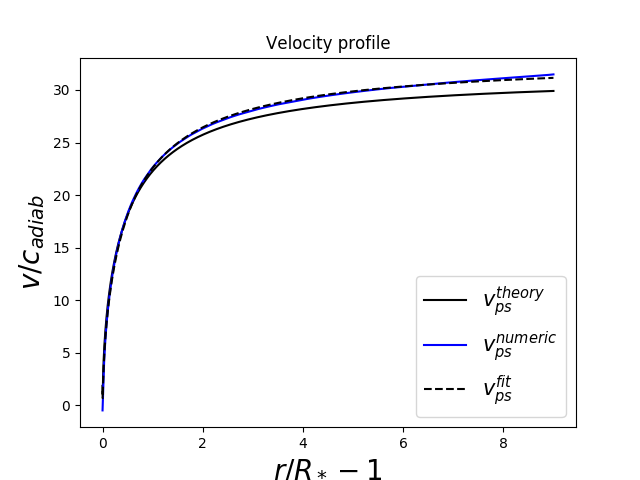
\includegraphics[width = \textwidth]{CAK_velocity_profile.png}
\caption{The velocity profile for the source point like star CAK wind. In dashed lines the initial conditions, in green the analytical steady state solution and in blue and red the solutions after 0.5 and 50 times $t = R_*/c_{adiab}$.}
\label{fig: CAK_PS_v}
\end{figure}

\begin{figure}
\centering
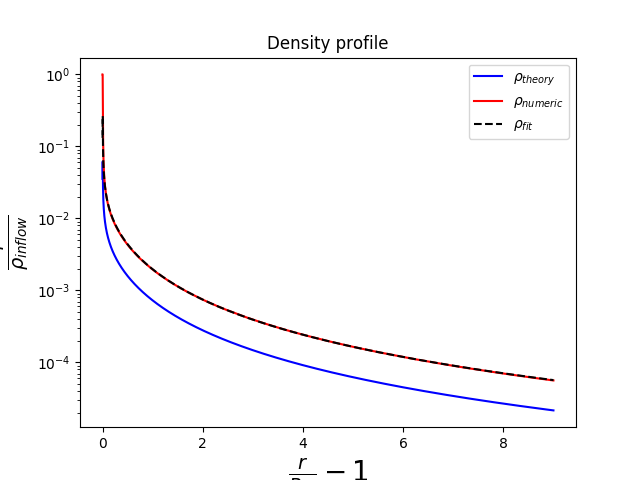
\includegraphics[width = \textwidth]{CAK_density_profile.png}
\caption{The density profile for the source point like star CAK wind. In dashed lines the initial conditions, in green the analytical steady state solution and in blue and red the solutions after 0.5 and 50 times $t = R_*/c_{adiab}$.}
\label{fig: CAK_PS_rho}
\end{figure}


%\begin{figure}
%\centering
%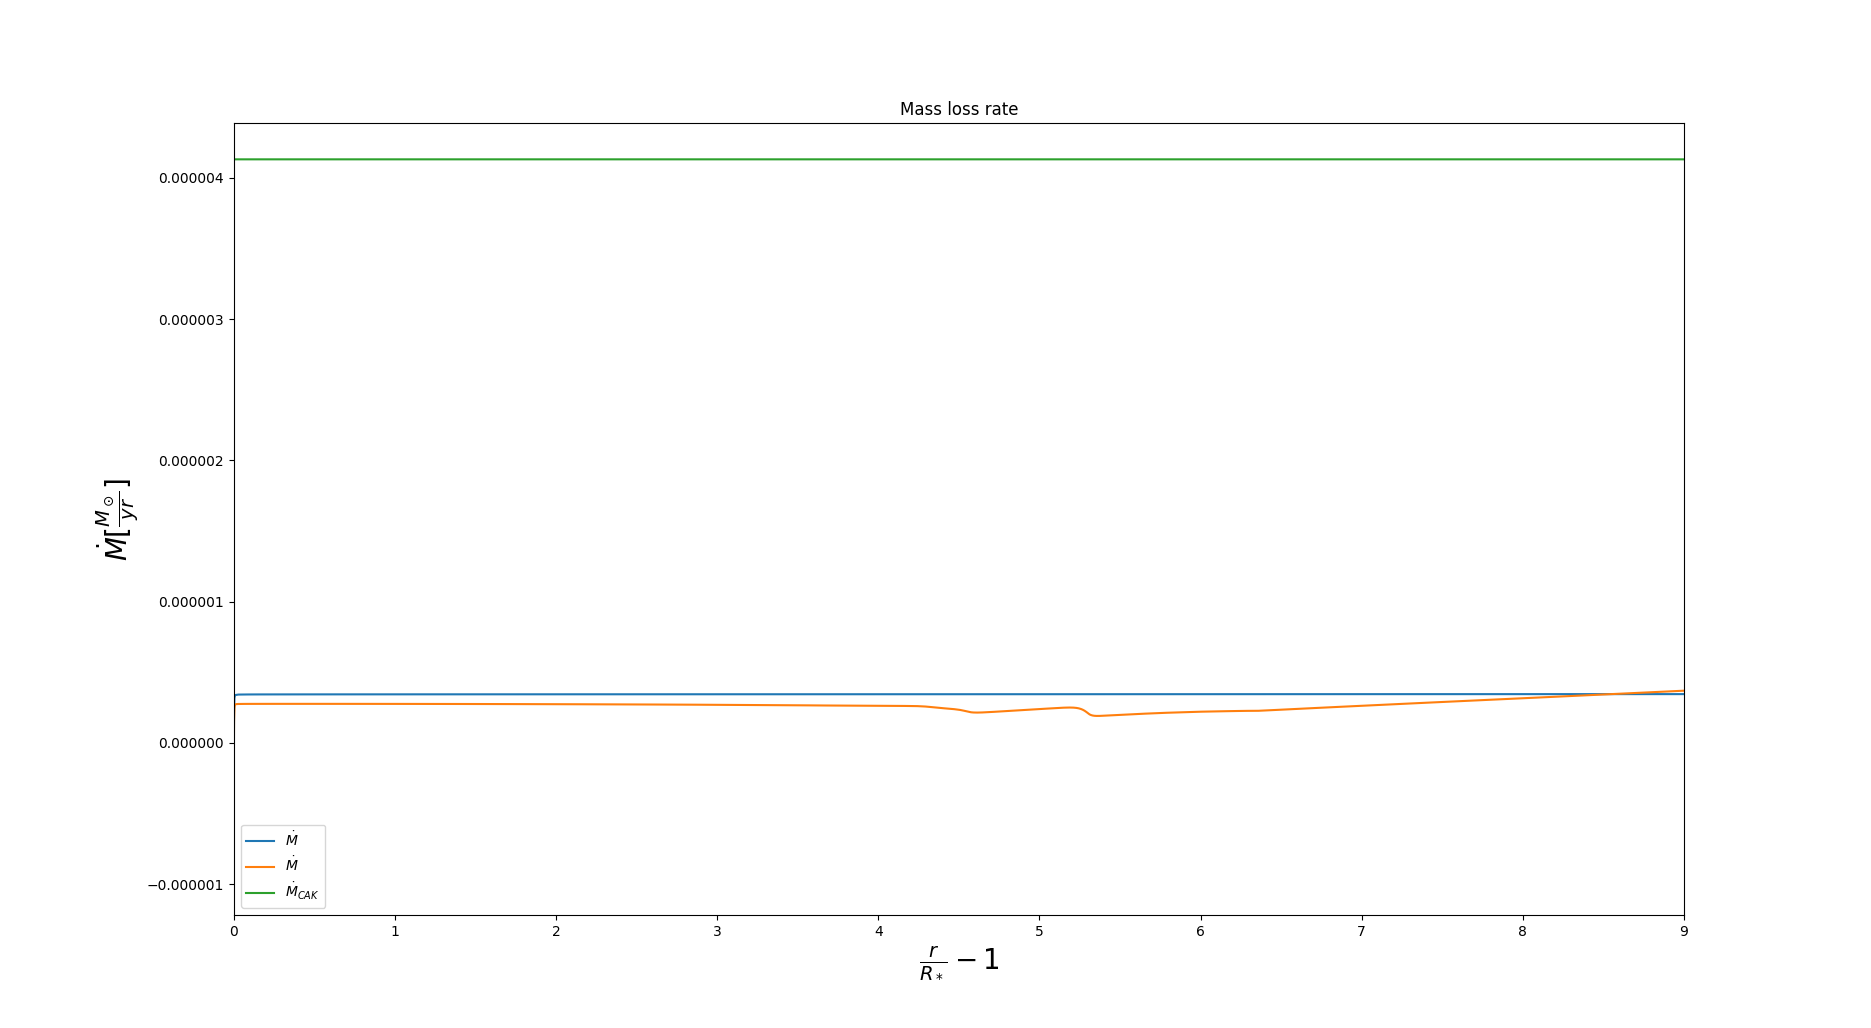
\includegraphics[width = \textwidth]{CAK_mass_loss.png}
%\caption{The mass loss rate profile for the source point like star CAK wind. In dashed lines the initial conditions, in green the analytical steady state solution and in blue and red the solutions after 0.5 and 50 times $t = R_*/c_{adiab}$.}\label{fig: CAK_PS_M_dot}
%\end{figure}

When accounting for the finite disk correction, the steady state velocity profile doesn't follow a $\beta = 0.5$ velocity law, results are shown in figures \ref{fig: CAK_PS_v} and \ref{fig: CAK_PS_rho}, the correction factor is plotted in figure \ref{fig: fd_factor}. 

\begin{figure}
\centering
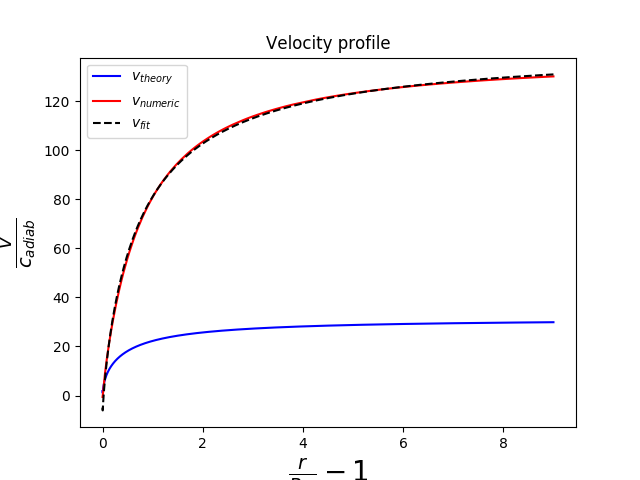
\includegraphics[width = \textwidth]{CAK_fd_velocity_profile.png}
\caption{The velocity profile for the finite disk corrected CAK wind. In dashed lines the initial conditions, in green the analytical steady state solution and in blue and red the solutions after 0.5 and 50 times $t = R_*/c_{adiab}$.}
\label{fig: CAK_fd_v}
\end{figure}

\begin{figure}
\centering
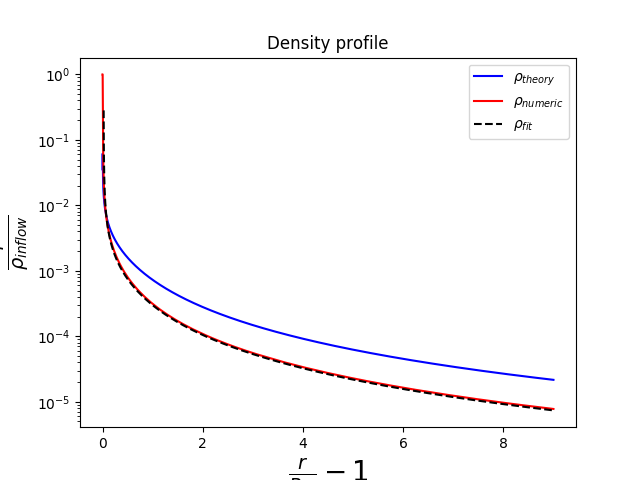
\includegraphics[width = \textwidth]{CAK_fd_density_profile.png}
\caption{The density profile for the finite disk corrected CAK wind. In dashed lines the initial conditions, in green the analytical steady state solution and in blue and red the solutions after 0.5 and 50 times $t = R_*/c_{adiab}$.}
\label{fig: CAK_fd_rho}
\end{figure}
%
%
%\begin{figure}
%\centering
%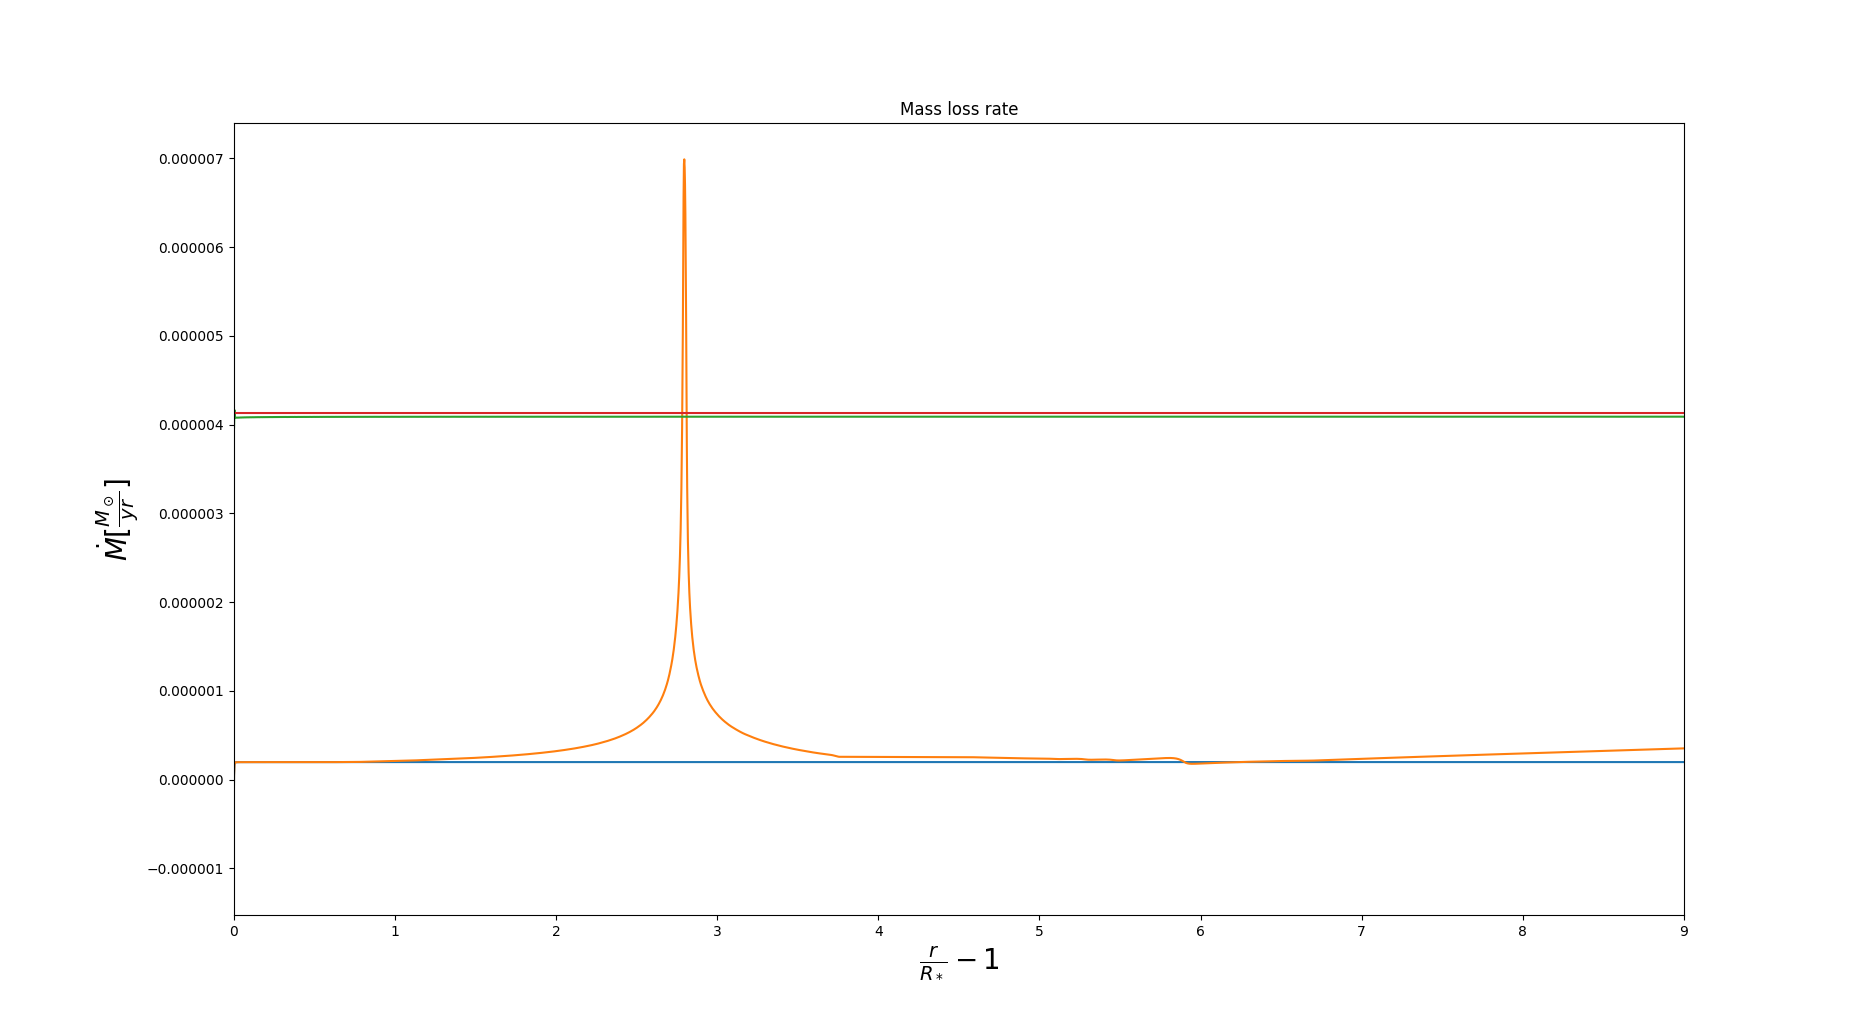
\includegraphics[width = \textwidth]{CAK_fd_mass_loss.png}
%\caption{The mass loss rate profile for the finite disk corrected CAK wind. In dashed lines the initial conditions, in green the analytical steady state solution and in blue and red the solutions after 0.5 and 50 times $t = R_*/c_{adiab}$.}
%\label{fig: CAK_fd_M_dot}
%\end{figure}

\begin{figure}
\centering
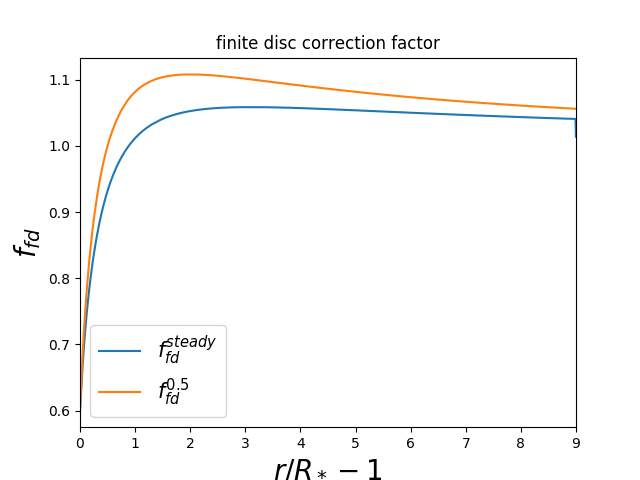
\includegraphics[width = \textwidth]{CAK_fd_factor.png}
\caption{•}
\label{fig: fd_factor}
\end{figure}


\section{Flux Limited Diffusion}
The diffusion model is first tested against some analytical results, these tests will give us knowledge on how accurately we can interpret the simulations of physical phenomena. The diffusion term and advection term are both tested separately by comparison to an exact solution and the photon tiring, radiative cooling and radiative heating source terms are tested together versus a Runge-Kutta solver of a simplified problem.

\subsection{Testcase 1: Advection and Diffusion}
The advection problem and the diffusion problem, solved by the already existing Riemann solver and the new ADI solver respectively can be tested by comparing them to simplified situation where an exact analytical solution can be found. The Riemann solver is nothing new, it's just a matter of checking the correct implementation in \texttt{MPI-AMRVAC}. The problem is tested on a numerical domain with constant density, a constant velocity, a constant gas energy density and an initial radiation energy density $E_0(x,y,t)$ given by:
\begin{align}
E_0(x,y,t) = 2 + \sin(2 \pi x) \sin(2 \pi y)
\end{align}
If diffusion and other source terms are ignored, the radiation field will evolve as
\begin{align}
E^{adv}(x,y,t) = 2 + \sin(2 \pi (x-v_x t)) \sin(2 \pi (y-v_y t))
\end{align}
If diffusion is switched on but the advection is ignored by fixing the velocity field to $\vec{0}$ every iteration, and the diffusion coefficient is chosen constant at $D = 1$, the field evolves as
\begin{align}
E^{diff}(x,y,t) = 2 + \exp(-8 \pi^2 t) \sin(2 \pi x) \sin(2 \pi y)
\end{align}

Function $E_0(x,y,t)$ describes a series of dots of more and less radiative energy, see figure \ref{fig: InitCond_test}. The numerical domain is chosen in such a way that there is one region of lower and one region of higher energy in each direction, $-0.5 \leq x \leq 0.5$, $0 \leq y \leq 1$. In time, the diffusion test runs until the amplitude of the dots diminish by two orders of magnitude $\exp(-8 \pi^2 t)  = 10^{-1}$ and the advection test tuns until a point has passed the computational domain twice $ \min(v_x, v_y) t = 2 $. Boundary conditions are set periodical. Computational result $\tilde{E}$ can be compared with the analytical results to define the residuals:
\begin{align}
RES^{adv} &= \left|\frac{\tilde{E}^{adv} - E^{adv}}{E^{adv}}\right| \\
RES^{diff} &= \left|\frac{\tilde{E}^{diff} - E^{diff}}{E^{diff}}\right| 
\end{align}

Which are plotted for different timesteps in figure \ref{fig: test_advection} and \ref{fig: test_diffusion} together with the numerical solutions $\tilde{E}^{adv}$ and $\tilde{E}^{diff}$


\begin{figure}
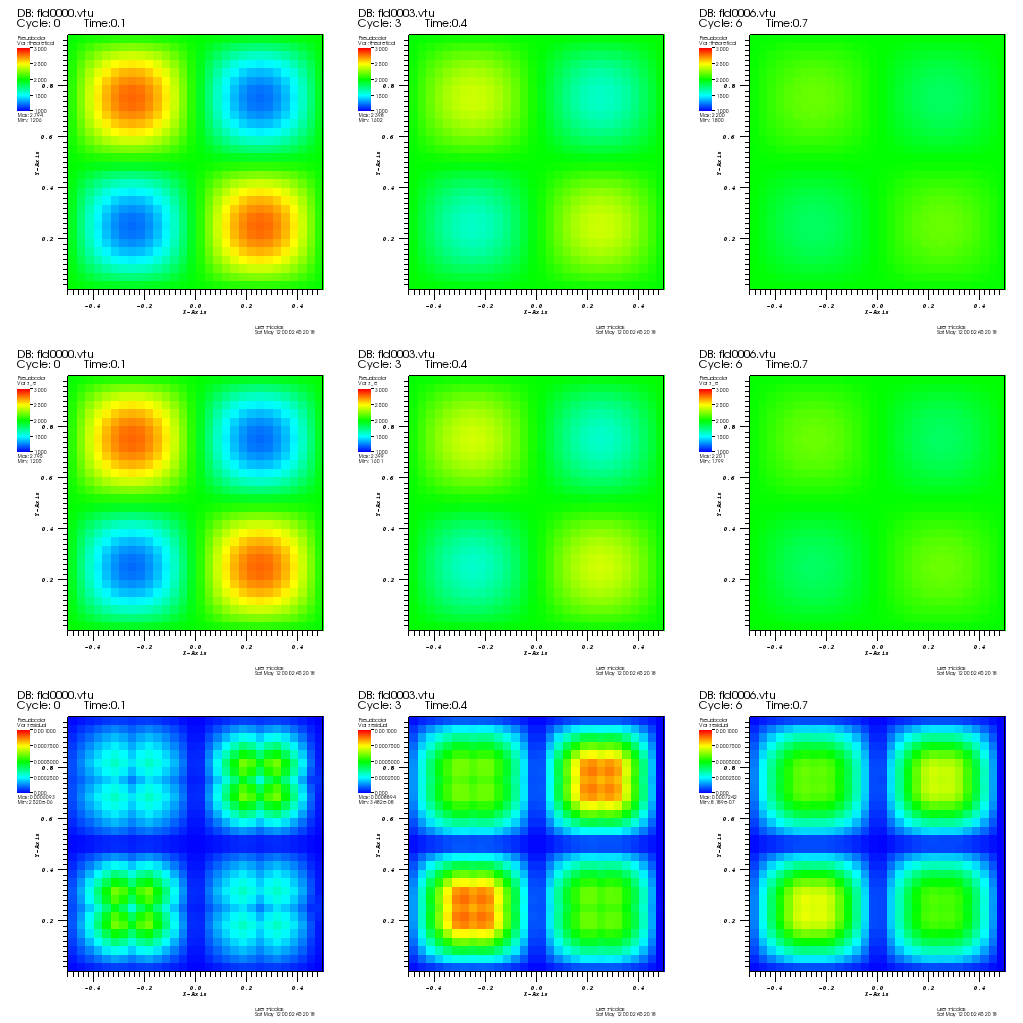
\includegraphics[width = \textwidth]{visit0001.png}
\label{fig: test_diffusion}
\caption{top: theoretical solution $E^{diff}$, middle: computed result $\tilde{E}^{diff}$ and bottom: residual $RES^{diff}$. Left: $0.1 t_0$, middle $0.4 t_0$ and right $0.7 t_0$. The scale goes from $1$ to $2$ for the upper two rows and form 0 to 0.01 for the bottom row.}
\end{figure}

\begin{figure}
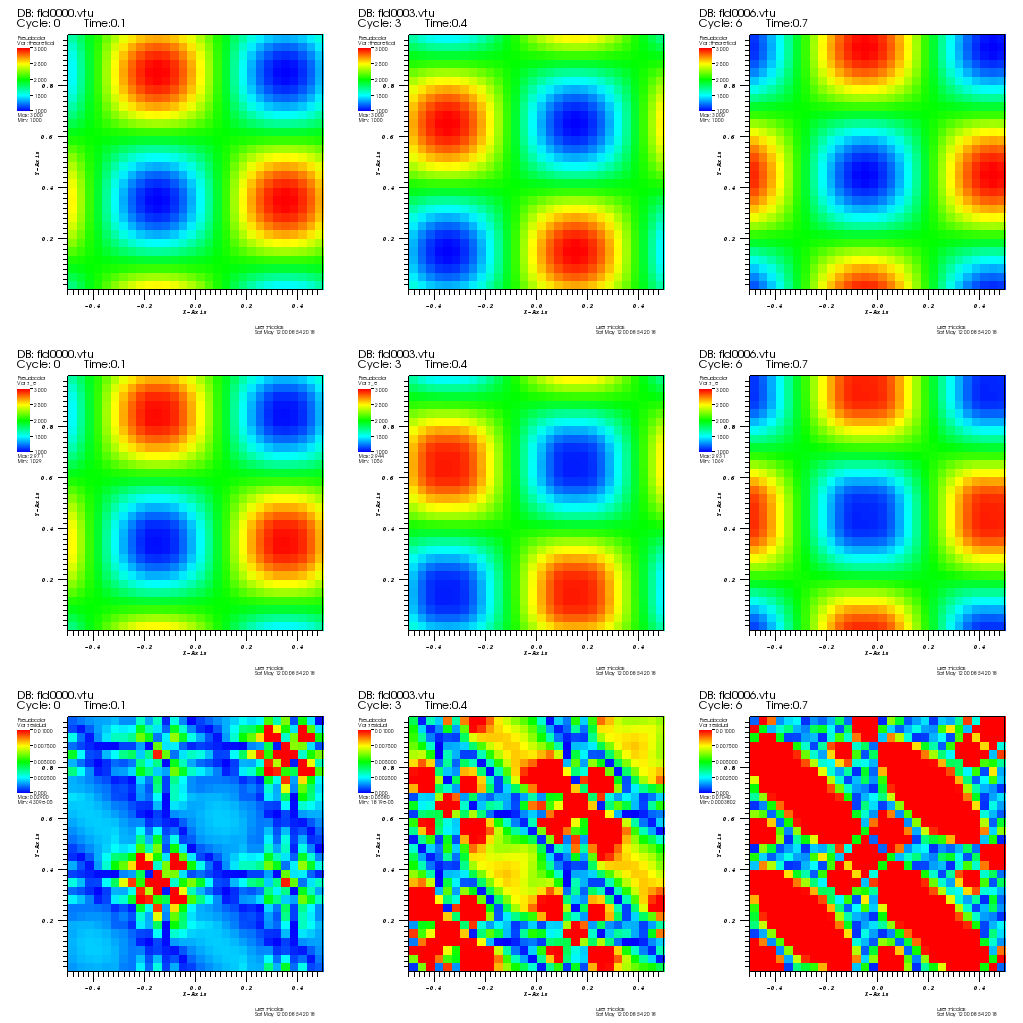
\includegraphics[width = \textwidth]{visit0002.png}
\label{fig: test_advection}
\caption{top: theoretical solution $E^{adv}$, middle: computed result $\tilde{E}^{adv}$ and bottom: residual $RES^{adv}$. Left: $0.1 t_0$, middle $0.4 t_0$ and right $0.7 t_0$. The scale goes from $1$ to $2$ for the upper two rows and form 0 to 0.001 for the bottom row.}
\end{figure}



\subsection{Testcase 2: Photon Tiring, Heating and Cooling}
To test the implicit bisection scheme used for adding the photon tiring, radiative heating and radiative cooling source terms, we make comparisons with an explicit Runge-Kutta solver. Of course this Runge-Kutta solver is not to be used in the actual code, because the time step chosen in the Runge-Kutta solver will be orders of magnitude smaller. The equation at hand is:
\begin{align}
\frac{d e}{dt} = c \rho \kappa E - 4 \rho \kappa \sigma T^4
\end{align}
Equivalently the test can be ran on the source terms for the radiative energy equation $\frac{dE}{dt} = - \vec{\nabla} \cdot \vec{v} P + 4\pi \kappa\rho B - c \kappa \rho E$ , where the photon tiring term would drop out due to the velocity field being zero.
Except for the gas energy density, all primitive variables ($\rho = \rho_0$, $\vec{v} = 0$ and $E = E_0$) are kept constant. The computational domain is taken as small as possible and radiative diffusion is switched off. \\

The system would be in radiative equilibrium when $c \rho \kappa E = 4 \rho \kappa \sigma T^4$. Using $T =  \frac{p}{\rho} \frac{m_p \mu}{k_b}= \frac{(\gamma - 1)e}{\rho} \frac{m_p \mu}{k_b}$, on can compute the equilibrium gas energy.
\begin{align}
e_{eq.} = \frac{\rho}{\gamma - 1} \frac{k_b}{m_p \mu}\left( \frac{c E}{4 \sigma} \right)^\frac{1}{4}
\end{align}
Different initial conditions are chosen for $e_0$ ranging from $10^2 e_{eq.}$ to $10^{-10} e_{eq.}$. Comparisons between the bisection method and a simple Runge-Kutta solver are plotted in figure \ref{fig: test_sourceterms}. Remember that the implicit bisection method uses a time step which is several orders of magnitude larger than the explicit Runge-Kutta method.

\begin{figure}
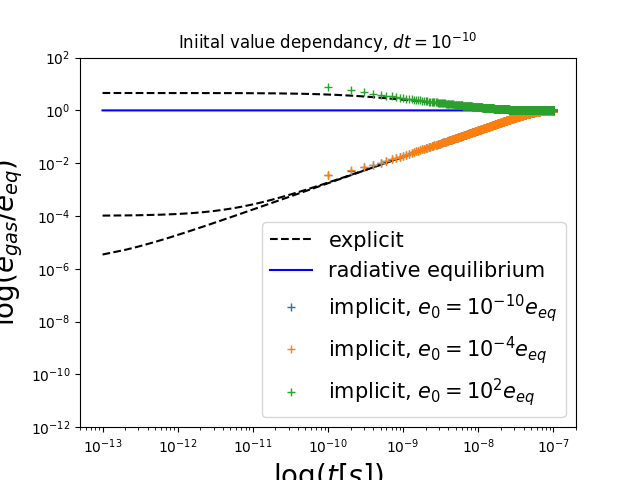
\includegraphics[width = \textwidth]{test_sourceterms.png}
\label{fig: test_sourceterms}
\caption{Comparison between the implicit method (red) and explicit method (black) for computing the radiation heating and cooling sourceterms. The gas energy evolves toward radiative equilibrium (blue) from different initial values. The time step for the implicit method is 3 orders of magnitude larger than the time step for the explicit method.}
\end{figure}

\begin{figure}
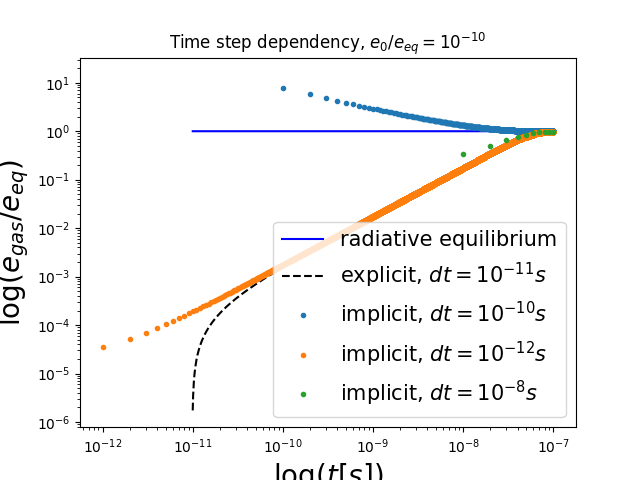
\includegraphics[width = \textwidth]{test_sourceterms_dt.png}
\label{fig: test_sourceterms}
\caption{Comparison between the implicit method (orange, blue, green) and explicit method (black) for computing the radiation heating and cooling sourceterms. The gas energy evolves toward radiative equilibrium (blue) with different time steps for the implicit method.}
\end{figure}

\subsection{Isothermal Thomson Atmosphere} \label{section: IsoAtm}
A first practical use for the FLD module is modelling a stellar atmosphere surrounding a massive star. For convenience, the atmosphere will be considered isothermal and plane parallel, so the flux in the initial condition and the gravitational acceleration are constant. Let's also assume the only absorption an emission is done by means of electron scattering (Thomson atmosphere), with a constant opacity $\kappa$. The model is done in 2D.\\

The initial conditions are crucial in stabilizing simulations. In an isothermal atmosphere, the density and gas pressure decay exponentially on the length of a scale height $H_{eff} = \frac{c_{sound}^2}{g_{eff}}$. Where $g_{eff} = g_{grav}(\Gamma - 1)$ is the sum of radiation and gravitational accelerations. 
\begin{align}
\rho(y) &= \rho_0 \exp \left( -\frac{y}{H_{eff}} \right) \\
 p(y)   &= p_0    \exp \left( -\frac{y}{H_{eff}} \right)
\end{align}

The velocity field is $\vec{0}$ everywhere. Boundary conditions $\rho_0$ and $p_0$ can be computed by defining the optical depth $\tau$. 
\begin{align}
\tau(y) = \int_\infty^{y} \kappa \rho dy  \label{eq: opt_depth}
\end{align}
Let $dm = \rho dy$, if this is substituted in \eqref{eq: opt_depth} we get an expression for the column mass in terms of opacity and optical depth:
\begin{align}
\frac{\tau}{\kappa} = \int_0^{m'} \rho dm
\end{align}


In a static medium, the gravitational and radiative acceleration of the gas is countered by the gas pressure gradient. Concerning the radiation field, one can make a similar statement . The radiative acceleration is countered by the radiation pressure gradient:
\begin{align}
\frac{dp}{dy} \frac{1}{\rho} &= \frac{dp}{dm} = -g_{grav}(1 - \Gamma) \label{eq: p_cond} \\
\frac{dP}{dy} \frac{1}{\rho} &= \frac{dP}{dm} = -g_{grav} \Gamma \label{eq: P_cond}
\end{align}
Manipulating equation \label{eq: p_cond} and substituting the expression for column mass leads to the following relation between optical depth and gas pressure:
\begin{align}
\int_0^{p_0} dp &= -g_{grav}(1 - \Gamma) \int_0^{m_0} dm
\end{align}
This expression can be integrated towards a value for $p_0$ at a given optical depth $\tau_0$. \eqref{eq: P_cond} And \eqref{eq: p_cond} can by divided by one another to get a relation between $dp$ and $dP$.
\begin{align}
p_0 = g_{eff} \frac{\tau_0}{\kappa} \\
dP = \frac{\Gamma}{\Gamma-1} dp
\end{align}
The gas energy density can be set from the gas pressure profile. Because of the plane parallel approximation, $\Gamma$ is constant as well and in the Eddington limit, $E=3P$. Now we have a boundary condition for the radiation energy field as well. The initial conditions are given by:
\begin{align}
\rho(y) &= g_{eff} \frac{\tau_0}{\kappa c_{sound}^2} \exp \left( -\frac{y}{H_{eff}} \right) \\
\rho \vec{v} &= \vec{0} \\
e &= \frac{\tau_0}{\kappa (\gamma - 1)} \exp \left( -\frac{y}{H_{eff}} \right) \\
E &= \frac{3 \Gamma}{1-\Gamma} \frac{\tau_0}{\kappa} \exp \left( -\frac{y}{H_{eff}} \right) \\
\end{align}

$\rho_0$ And $p_0$ are also used as lower boundary conditions for density and gas energy during the simulations. The  boundary condition for the $x$-component of the velocity is $0$ and the one for the $y$-component is set with the help of the steady state continuity equation $\partial_y(v_y \rho) = 0$. In a discrete form this can be written as:
\begin{align}
v_{y,0} = \frac{v_{y,1} \rho_1}{\rho_0}
\end{align}
Where the value in the first ghostcell is indicated with index $_0$.\\
For the radiation energy it is not only important that $E$ has the correct value, even more important is the value for $F_y$. Lets begin by writing down a discrete form of the initial conditions:
\begin{align}
E_{i+1} &= \frac{3 \Gamma_{i+1}}{1-\Gamma_{i+1}}_{i+1} \\
\Gamma_{i+1} &= \frac{1}{1 + \frac{3 p_{i+1}}{i+1}} \label{eq: Gamma1}
\end{align}
Using the defenition of the Eddington parameter $\Gamma_{i+1} = \frac{\kappa F_{y,i+1}}{c g_{grav}}$ and a discrete form of the fld closure relation equation \eqref{eq: fld_closing} $F_{i+1} = -\frac{c \lambda_{i+1}}{\kappa \rho_{i+1}} \frac{E_{i+2} + E_{i}}{2 \Delta x}$ one can write down another expression for $\Gamma$:
\begin{align}
\Gamma_{i+1} = \frac{\lambda_{i+1}}{g_{grav}\rho_{i+1}}\frac{E_i + E_{i+2}}{2 \Delta x} \label{eq: Gamma2}
\end{align}

Eliminating the Eddinton parameter in equations \ref{eq: Gamma1} and \eqref{eq: Gamma2} makes it possible to give an elegant expression for $E_i$:
\begin{align}
E_i = E_{i+2} + \frac{2 \Delta x}{1 + \frac{3 p_{i+1}}{i+1}}  \frac{g_{grav} \rho_{i+1}}{\lambda_{i+1}}  
\end{align}
This expression gives a radiation energy field which leads to a physical flux when calculating it from the closure relation. On the lower boundary, a "no inflow" condition is used. This means that the gradient of the densities is preserved as long as it is smaller than $0$. Periodic boundary conditions are used on the sides. \\ STILL HAVE TO CHECK LAST STATEMENT!!!\\

After every time step, the gas energy density is set as function of the gas density and momentum to match the constant temperature structure to keep the atmosphere isothermal. This is done using the inner boundary condition module in \texttt{MPI-AMRVAC}.\\


The parameters defining the physics of the system are the Eddington parameter $\Gamma$, the optical depth at the lower boundary $\tau_0$ and the sound speed $c_{sound}$. The Eddington parameter contains information about the mass, luminosity and radius of the star, it determines whether the atmosphere will be blown away, collapsing in on itself or relax in a steady state. $\tau_0$ Sets the physical lower boundary of the numerical domain. A high value means the model starts at in a high density environment near the core, a low value means the model simulates the outermost boundaries of the star. The sound speed determines the temperature of the atmosphere and the velocity at which waves can travel. Together with the Mass which sets the gravitational field, the sound speed also determines the scale height of the gas. \\

Calculations are done on a Cartesian grid, with the y-direction parallel to the radius of the star.The mass of the star is chosen at $M_* = 50 M_\odot$. Using Leavit's law, we get a luminosity for a typical $50M_\odot$ star of $L_* = ... L_\odot$ and an Eddington parameter $\Gamma = ...$. The calculation domain begins at $\tau_0 = ...$ and the grid resolves about $...$ scale heights in the y-direction and $...$ in the x-direction. The resolution of the grid is chosen such that there are $...$ cells per scale height. The simulation stops after $...$ times the hydrodynamical timescale, this is the time needed for a sound wave to travel across the computational domain. 

\subsubsection{constant flux discrepancy}

\subsection{Strange mode instabilities}

\subsection{Non-isothermal evolution?}
This section describes the result of evolving the initial conditions described in section \ref{section: IsoAtm} without the isothermal conditions. So now, also the radiation heating and cooling source terms are taken into account for the gas energy equation. Snapshots in the simulation are compared visually to snapshot from the isothermal atmosphere.

\subsubsection{comparison to mesa structure}

